\documentclass{article}

\usepackage{times}
\usepackage{uist}

\usepackage{graphicx}
\usepackage{caption}
\usepackage{subcaption}

\begin{document}

% --- Copyright notice ---
\conferenceinfo{UIST'12}{October 7-10, 2012, Cambridge, MA, USA}
\CopyrightYear{2012}
\crdata{978-1-xxxx-xxxx-x}

% Uncomment the following line to hide the copyright notice
% \toappear{}
% ------------------------

\bibliographystyle{plain}

\title{Demo: Spatial augmented reality for \\
       physical drawing}

%%
%% Note on formatting authors at different institutions, as shown below:
%% Change width arg (currently 7cm) to parbox commands as needed to
%% accommodate widest lines, taking care not to overflow the 17.8cm line width.
%% Add or delete parboxes for additional authors at different institutions. 
%% If additional authors won't fit in one row, you can add a "\\"  at the
%% end of a parbox's closing "}" to have the next parbox start a new row.
%% Be sure NOT to put any blank lines between parbox commands!
%%


\author{
\parbox[t]{9cm}{\centering
	     {\em Jeremy Laviole}\\
	     Univ. Bordeaux, LaBRI, UMR 5800, F-33400 Talence, France.\\
         CNRS, LaBRI, UMR 5800, F-33400 Talence, France.\\
	     Inria, F-33400 Talence, France.\\
	     laviole@labri.fr \vspace*{-0.5cm}}
\parbox[t]{9cm}{\centering
	     {\em Martin Hachet}\\
	     Inria, F-33400 Talence, France.\\
	     LaBRI, UMR 5800, F-33400 Talence, France.\\
	     martin.hachet@inria.fr}
}


\maketitle

\abstract
Spatial augmented reality (SAR) makes possible the projection of virtual environments into the real world. In this demo, we propose to demonstrate our SAR tools dedicated to drawing. 
From the most simple tools: the projection on virtual guidelines enabling to trace lines and curves  to more advanced techniques enabling stereoscopic drawing through the projection of a 3D scene. This demo presents how we can use computer graphics tools to ease the drawing, and how it will enable new kinds of physical drawings. 

\classification{H5.1 [Information interfaces and presentation]:
Multimedia Information Systems. - Artificial, augmented, and virtual realities}

\terms{Design, Human Factors}

\keywords{Spatial augmented reality, user interfaces, arts, interactive projection}


\tolerance=400 
  % makes some lines with lots of white space, but 	
  % tends to prevent words from sticking out in the margin

\section{INTRODUCTION}

Spatial augmented reality was first created to project textures and illuminations to physical objects~\cite{raskar1999table}. Nowadays, it is mostly exposed for advertising, featuring projection on large building and commonly called "projection mapping". 
But the size of the projector decreases and many uses of embedded SAR are  imagined~\cite{mistry2009sixthsense}. 
Entertainment will benefit largely from SAR, the inclusion of digital games into the real world changes completely the aspect of it~\cite{wilson2007depth}~\cite{jones2010build}.

Drawing is one of the first activity we learn to do. It is a direct expression method and a pleasant activity. It leads to a unique result, which can represent from minutes to years of work. 

In this demonstration, we propose to use SAR for the creation of physical drawings (on paper); in opposition with digital drawings (in memory). By the use of computer graphics tools we enable easier and faster drawings. It is an evolution of the demonstration we did described in~\cite{laviole:2012} which was oriented for a general public exhibition. Here we focus on the tools and challenges of integrating digital information for drawing, and we will present our latest tools.


\section{SAR for drawing}
\subsection{Firsts steps}

We present one of the firsts SAR application dedicated to drawing. The first application we propose is the projection of images such as photos on tracked sheets of paper. The piece of paper is surrounded by markers and is tracked by a camera mounted on a projector (procam), as illustrated in Figure~\ref{fig:system}.
This kind of overhead projection allows any kind of paper and not intrusive. Any drawing or painting tools can be used to copy or use the projected image to create a drawing. Our system focuses on the precision of the projection, it relies on a precise estimation of the camera and projector internal parameters\cite{audet2010direct}. 

\begin{figure}[!b]
\centering 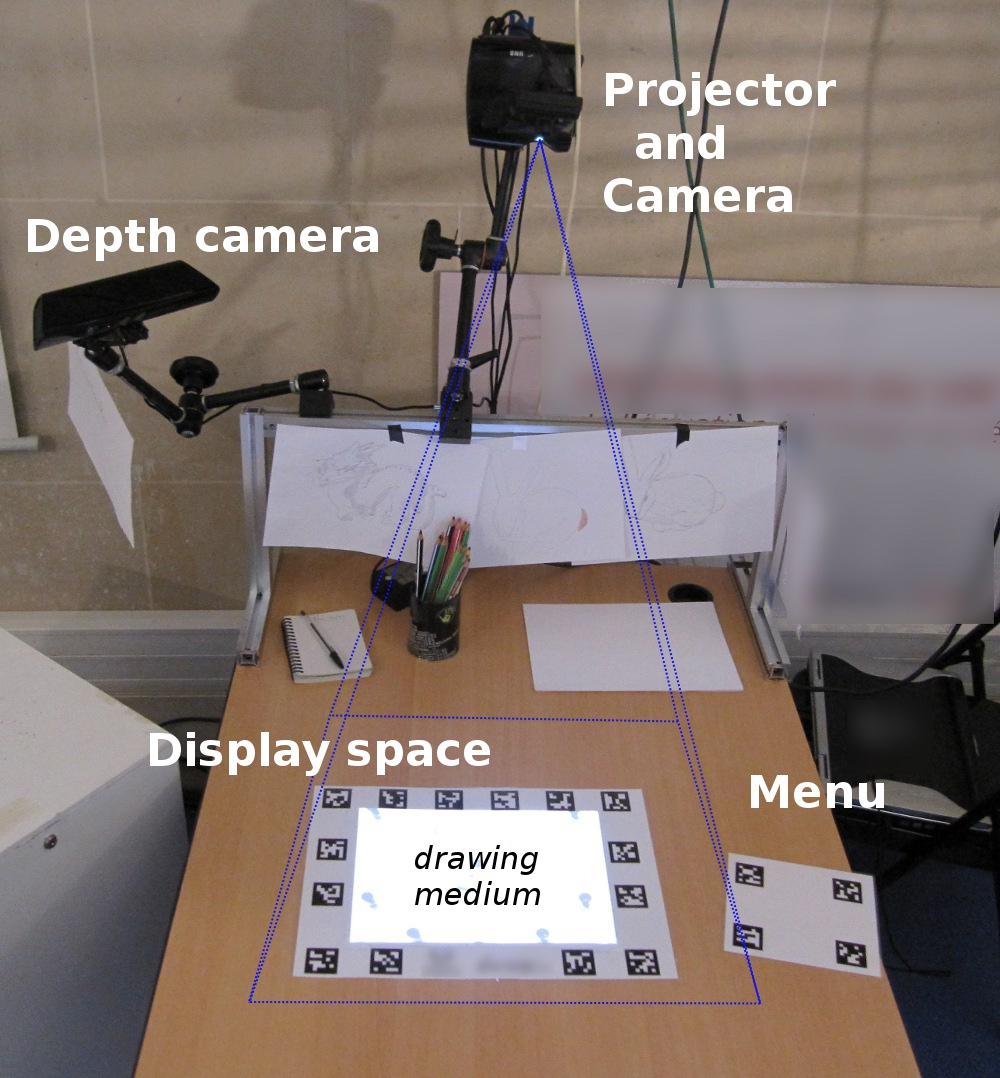
\includegraphics[width = 70mm]{global}
\caption{View of the system during a public exhibition.} 
\label{fig:system}
\end{figure}

\subsection{Interactivity}

The procam system is made interactive by the addition of a depth camera. The depth camera makes the table and projected elements reactive to touch and 3D pointing events, illustrated in Figure~\ref{fig:inter}. We took advantage of this to provide direct manipulation of the projection and to add menus on a separated paper sheet. The separation of the menu and the drawing space avoids many undesired selections and allows to the user to take full advantage of the projection space while drawing. Additionally, we added a pen and tablet device to get a precise input from the user. 

\subsection{Merge with traditional drawing software}
Our goal is to improve the physical creation, and the easiest way to use digital tools for physical creation is to directly integrate them with our system. In order to do this we added a high resolution camera which takes pictures of the drawing and saves them on the disk. The picture can be opened in any drawing software, for our examples we used The Gimp. In the drawing software, the elements to project can be created in a dedicated layer; obviously the physical drawing does not need to be projected only the added elements have to be saved. The whole process is semi-automatic, pressing a button in the projection software saves the current drawing, and pressing another one loads the projection from the disk. Figure~\ref{fig:velo} illustrate an example of drawing plus projection.

\subsection{Projection of a 3D scene}
Because many drawings use models, we wanted to transpose the same possibilities for our system. 
Setting a scene consists in choosing a point of view, and setting the lighting conditions for the desired scene.
The scene projection is made to be simple to manipulate and visualize, consequently for now the manipulations are constrained. 
The virtual objects are placed on the paper sheet, and can be manipulated though the touch or the tangible interfaces. Moreover, the user can change the lighting conditions by setting directly the light location in the 3D scene by using the 3D pointing solution. Once the point of view of the 3D scene is set, the user can save a screen shot of the application and use is to draw as described before. A scene containing the 3D model of a physical dragon is illustrated in Figure~\ref{fig:inter}.


\begin{figure}[!h]
        \begin{subfigure}[b]{4.2cm}
                \centering
                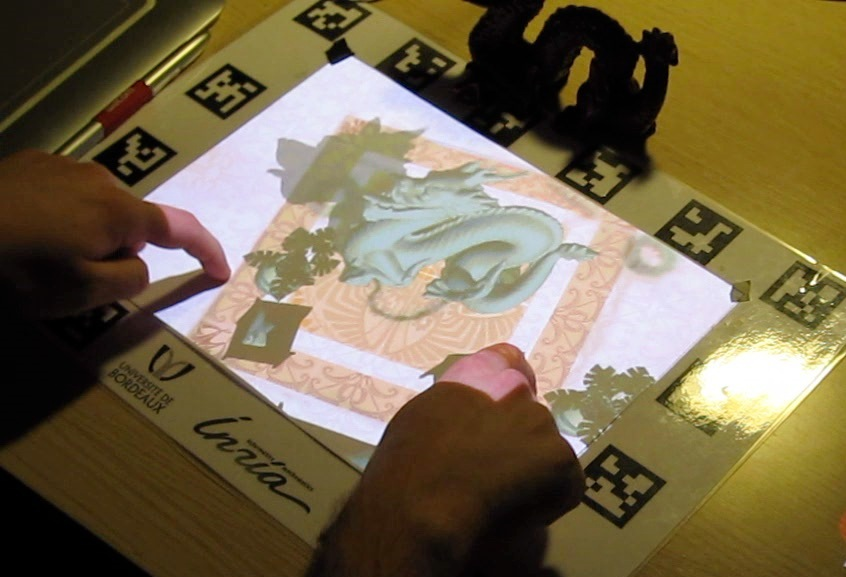
\includegraphics[width=4.2cm]{Still2}
                \caption{Touch}
                \label{fig:touch}
        \end{subfigure}%
        ~ %add desired spacing between images, e. g. ~, \quad, \qquad etc. 
          %(or a blank line to force the subfigure onto a new line)
        \begin{subfigure}[b]{0.25\textwidth}
                \centering
                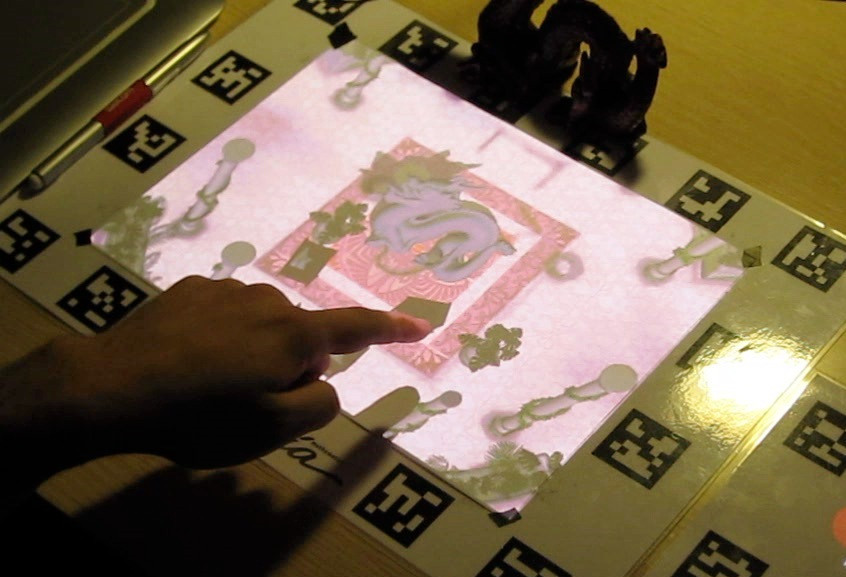
\includegraphics[width=4.2cm]{Still1}
                \caption{3D pointing}
                \label{fig:point}
        \end{subfigure}
        \caption{The user can interact by touching or pointing in the air.}
        \label{fig:inter}
\end{figure}

\subsection{Extension to stereoscopic drawing} 
The view of the 3D scene provides a good perception of depth and shapes. This perception is even better using a stereoscopic visualization. After extending the visualization, we extended our application to create stereoscopic drawings. The generated left and right images lead to two different drawings. In order to visualize and edit the drawings, we also created dedicated tools to  capture the two drawings,and combine them to get an instantaneous stereoscopic preview. Unfortunately for the demonstration, the creation of two drawings providing good bumping effects requires time and takes much more space (3 drawing spaces), the demonstration of this tool will be harder to give.  

\begin{figure}[!h]
        \begin{subfigure}[b]{0.20\textwidth}
                \centering
                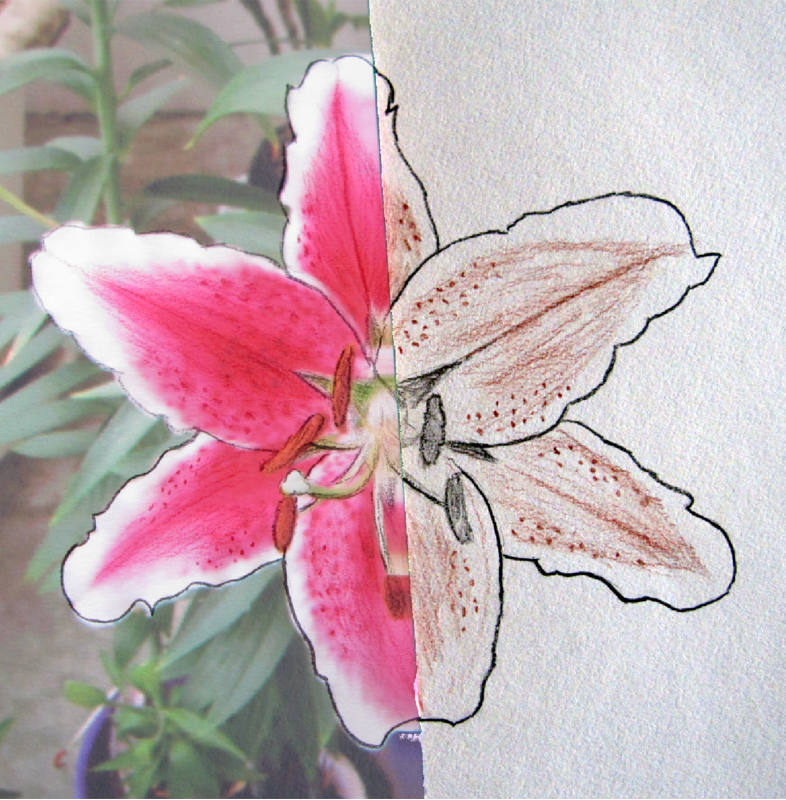
\includegraphics[height=3.4cm]{lys}
                \caption{Lily flower.}
                \label{fig:lys}
        \end{subfigure}%
        ~ %add desired spacing between images, e. g. ~, \quad, \qquad etc. 
          %(or a blank line to force the subfigure onto a new line)
        \begin{subfigure}[b]{0.25\textwidth}
                \centering
                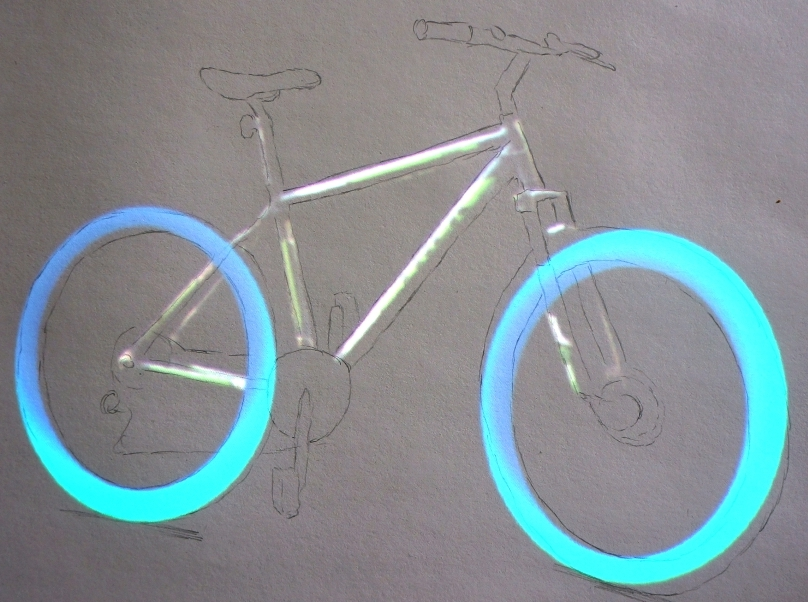
\includegraphics[height=3.4cm]{velo2}
                \caption{Bike}
                \label{fig:velo}
        \end{subfigure}
        \caption{Blending projection and physical drawing creates new visual experiences.}\label{fig:drawings}
\end{figure}


\section{Conclusion}
The creation of the tools described above involved the creation of many testing tools. Some of them are games and musical applications, which we generally enjoy to demonstrate and play with. 
This demonstration proposes a new way to consider the use of computers. By providing tools to ease and fasten the drawing, the visitors could enjoy the simple pleasure of drawing. We keep the natural elements of drawing, and we provide tools from computer graphics to enhance creativity.

\bibliographystyle{abbrv}
\bibliography{paper}

\end{document}